\begin{mainquestion}{pmosgateresistor}{PMOS Amplifier with Gate Resistor}

In the circuit shown below, the PMOS transistor has $V_{tp} = -0.6\ \text{V}$, $V_{A} = -100\ \text{V}$, and operates with $V_{D} = 5\ \text{V}$. Note the 3 MΩ gate resistor, which is another way to bias a CS stage, used here in addition to the current source. You may assume that any channel length modulation does not appreciably affect the DC biasing.

\begin{center}
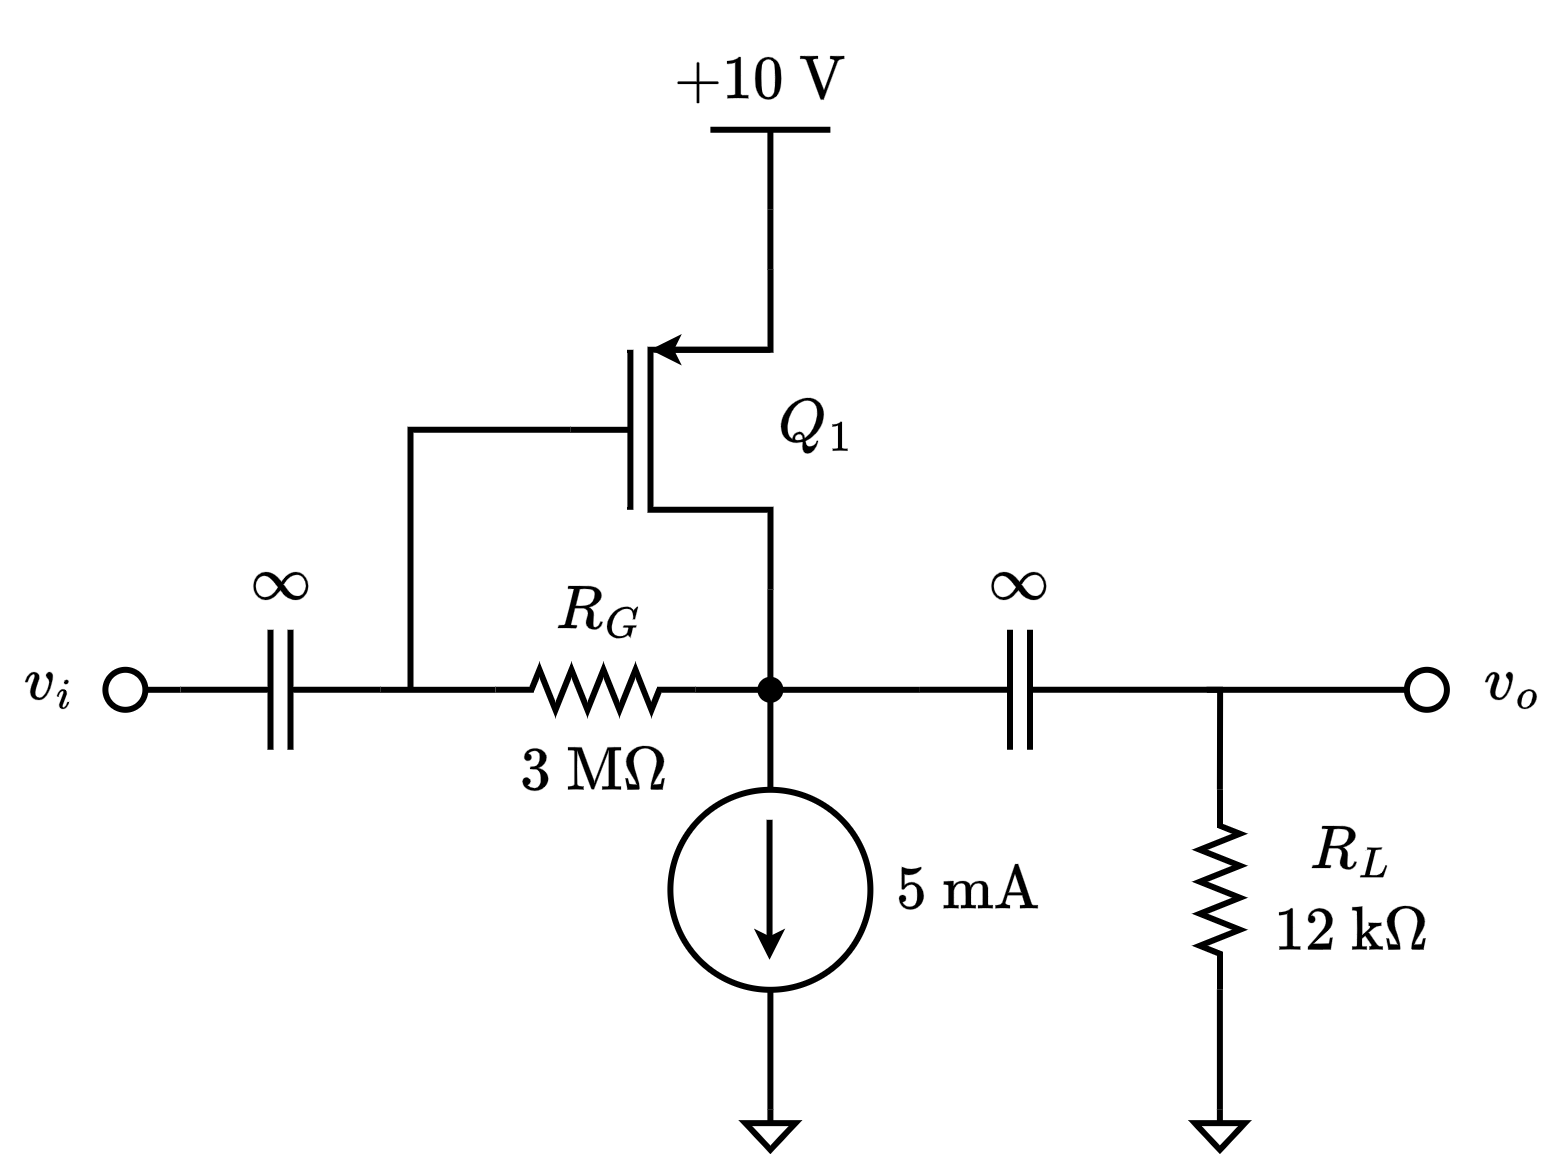
\includegraphics[width=4in]{circuit.png}
\end{center}

\begin{partquestion}{smallsignal}{Draw the small-signal equivalent circuit for this transistor amplifier. Be sure to label the input and output voltages as well as the source, gate and drain locations on the schematic. Calculate all parameters/component values used in your equivalent circuit that were not given in the problem.}
\begin{answer}
The small signal equivalent circuit is shown below.

\begin{center}
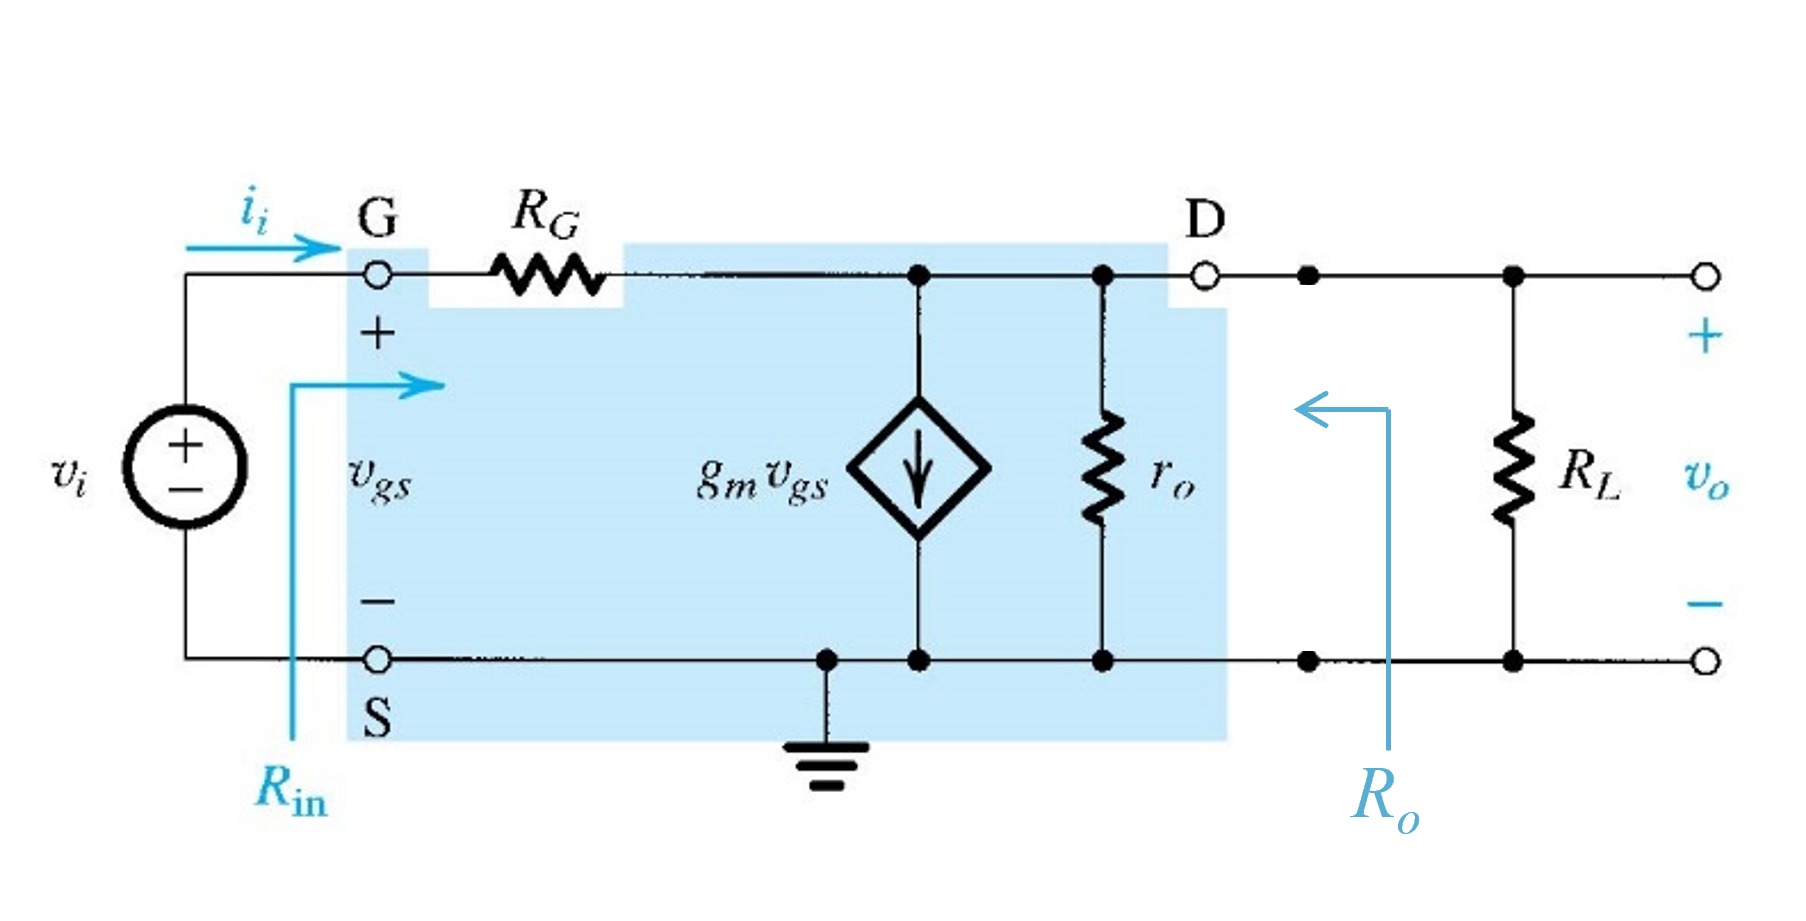
\includegraphics[width=5in]{../v0/smallsignal.png}
\end{center}

We can calculate the parameters not given in the problem as:

\[
g_{m} = \frac{2I_{D}}{\left|V_{OV}\right|} = \frac{2I_{D}}{V_{S} - V_{G} - \left|V_{tp}\right|}
\]

Note $V_{S} = \qty{10}{\volt}$ and $V_{G} = V_{D}$ since there is no DC current flowing through $R_{G}$ due to the capacitors and the transistor gate. This gives:

\begin{align*}
    g_m &= \frac{2 I_D}{V_{S} - V_D - |V_{tp}|} \\
    &= \frac{2 \cdot 5}{10 - 5 - |-0.6|} \\
    &= \qty{2.27}{\milli\siemens}
\end{align*}

The drain-to-source resistance is:

\[
r_{o} = \frac{\left|V_{A}\right|}{I_{D}} = \frac{|-100|}{5} = 20\ \text{k}\Omega.
\]
\end{answer}
\end{partquestion}

\begin{partquestion}{resistance}{What is the input resistance of the amplifier? What is the output resistance?}
\begin{answer}
The presence of the resistor between gate and drain makes this calculation less trivial than some configurations. Here, we use KCL at the drain to give:

\begin{align*}
    i_i &= g_m v_{gs} + \frac{v_o}{r_o \parallel R_L} \\
    &= g_m v_i + \frac{v_o}{r_o \parallel R_L} \\ 
\end{align*}

And use KVL to find:

\[
i_{i} = \frac{v_{gs} - v_{o}}{R_{G}} = \frac{v_{i} - v_{o}}{R_{G}}
\]

Solving for $v_{o}$ in the second equation gives $v_{o} = v_{i} - i_{i}R_{G}$ which plugs back into the first result to yield:

\[
i_{i} = g_{m}v_{i} + \frac{(v_{i} - i_{i}R_{G})}{(r_{o} \parallel R_{L})}
\]

\[
i_{i}\left(1 + \frac{R_{G}}{r_{o} \parallel R_{L}}\right) = v_{i}\left(g_{m} + \frac{1}{r_{o} \parallel R_{L}}\right)
\]

Since $R_{\text{in}} = \frac{v_{i}}{i_{i}}$ we can write:

\begin{align*}
    R_{in} &= \frac{1 + \frac{R_G}{r_o \parallel R_L}}{g_m + \frac{1}{r_o \parallel R_L}} \\
    &= \frac{r_o \parallel R_L + R_G}{g_m (r_o \parallel R_L) + 1} \\
\end{align*}

Substituting in values found in part (a) gives:

\begin{align*}
    R_{in} &= \frac{\qty{20}{\kilo\ohm} \parallel \qty{12}{\kilo\ohm} + \qty{3}{\mega\ohm}}{(\qty{2.27}{\milli\siemens}) (\qty{20}{\kilo\ohm} \parallel \qty{12}{\kilo\ohm}) + 1} \\
    &= \frac{\qty{3.008}{\mega\ohm}}{18.05} \\
    &= \qty{167}{\kilo\ohm}
\end{align*}

Looking at the small-signal equivalent circuit, the output resistance is simpler to calculate than the input resistance. First, the load resistance is removed prior to calculation, and the input is set to zero, so $v_{gs} = 0$, which means the current source has no current flow and becomes an open circuit. It follows immediately, that:
\begin{align*}
    R_o &= R_G \parallel r_o \\
    &= \frac{3000 \cdot 20}{3000 + 20} \unit{\kilo\ohm} \\
    &= \qty{19.8}{\kilo\ohm}
\end{align*}
\end{answer}
\end{partquestion}

\begin{partquestion}{voltgain}{What is the voltage gain $A_{v} = \frac{v_{o}}{v_{i}}$? How much does your calculation change if you assume $R_{G} \rightarrow \infty$?}
\begin{answer}
In part (b), we found:

\[
i_{i} = g_{m}v_{i} + \frac{v_{o}}{r_{o} \parallel R_{L}}
\]

and

\[
i_{i} = \frac{v_{i} - v_{o}}{R_{G}}.
\]

Equating these gives:

\begin{align*}
    \frac{v_i - v_o}{R_G} &= g_m v_i + \frac{v_o}{r_o \parallel R_L} \\
    v_i\left(\frac{1}{R_G} - g_m\right) &= v_o + \left(\frac{1}{R_G} + \frac{1}{r_o \parallel R_L}\right) \\
\end{align*}

Since $A_{v} = \frac{v_{o}}{v_{i}}$, we can rearrange to write:

\begin{align*}
    A_v &= \frac{\frac{1}{R_G} - g_m}{\frac{1}{R_G} + \frac{1}{r_o \parallel R_L}} \\
    &= \frac{r_o \parallel R_L - g_m R_G(r_o \parallel R_L)}{r_o \parallel R_L + R_G} \\
    &= \frac{20 \parallel 12 - (2.27) (3000) (20 \parallel 12)}{20 \parallel 12 + 3000} \\
    &= -17.00 \\
\end{align*}

When $R_{G} \rightarrow \infty$, this becomes:

\begin{align*}
    A_v &= \frac{-g_m R_G (r_o \parallel R_L)}{R_G} \\
    &= -g_m (r_o \parallel R_L) \\
    &= -(2.27) (20 \parallel 12) \\
    &= -17.05
\end{align*}

which is a change of only 0.26\% (in absolute gain). Either way, the answer is pretty close to $-17$! What else would it have been?
\end{answer}
\end{partquestion}

\end{mainquestion}
